% ----------------------------------------------------------------------
% CAPÍTULO 3 - RESULTADOS OBTIDOS
% ----------------------------------------------------------------------

As representações gráficas dos resultados dos experimentos estão representadas na Figura 1. No eixo horizontal está representado o número de épocas de treinamento das redes. No eixo vertical é mostrada a acurácia. As cores representam cada batch size usado. As colunas da matriz de gráficos representam as redes usadas e as linhas da matriz representam os learning rates usados.  

Os resultados mostram que não foram observadas acurácias muito distintas quando alterava-se o batch size, é possível verificar que, em vários momentos, os pontos ficaram sobrepostos.

Quanto ao learning rate, o único cenário que mostra algum efeito da taxa é aquele com valor igual 0.01 para a rede Lenet; este cenário apresenta uma acurácia crescente conforme aumenta-se o número de épocas do treinamento. Nos demais cenários foi verificada uma considerável estabilidade dos resultados da acurácia, não sendo verificado uma melhora substancial no aumento de épocas do treinamento da rede.

Quanto aos tempos de ajuste, a rede Lenet5 se mostrou a mais rápida. A rede Alexnet levava cerca de 10 minutos por modelo. Para a rede pré treinada Xception, houve casos que demoararam mais de 30 minutos para execução dos cenários em 100 épocas, os cenários com treinamento maior que 100 épocas sequer puderam ser obtidos devido ao tempo. Já a rede pré treinada MobileNetV2 apresentou tempos similares ao Lenet5.

Quanto às acurácias em cada rede, os melhores resultados foram observados para a rede AlexNet, que apresentou acurácias acima de 0.9. A rede Lenet5 e o Xception apresentaram acurácias em torno de 0.8. Já a rede MobileNetV2 apresentou o pior resultado, com uma acurácia em torno de 0.4. A tabela 1 mostra as acurácias médias observadas para cada cenário. 

\begin{table}[h]
\centering
\begin{tabular}{c|cccc}
\hline
Modelo        & Lenet5 & AlexNet & Xception & MobileNetV2 \\ \hline
Média         & 0.79   & 0.93    & 0.77     & 0.40        \\
Desvio padrão & 0.05   & 0.02    & 0.007    & 0.005       \\ \hline
\end{tabular}
\caption{Média e desvio padrão das acurácias de cada rede utilizada.}
\label{tab:my-table}
\end{table}

Com isso, a estratégia de seleção do melhor modelo para prosseguimento das análises se deu através do filtro dos modelos com acurácia acima de 0.9, com menor número de épocas, maior batch size e maior taxa de aprendizado. Este modelo foi um AlexNet com 100 épocas, learning rate de 0.5 e batch size de 256. A matriz de confusão deste modelo é apresentada na tabela 2.

\textbf{MATRIZ DE CONFUSÃO}

Este mesmo modelo foi ainda utilizado para extração de características e geração de novas bases de treino e teste para aplicação de um modelo de regressão logística para classificação dos meses manuscritos. Este modelo apresentou uma acurácia de 0.49 e a matriz de confusão é apresentada na tabela 3.

\begin{table}[h]
\centering
\begin{tabular}{c|cccccccccccc}
\textbf{}    & \textbf{Jan}                     & \textbf{Fev}                     & \textbf{Mar}                     & \textbf{Abr}                     & \textbf{Mai}                    & \textbf{Jun}                    & \textbf{Jul}                     & \textbf{Ago}                     & \textbf{Set}                     & \textbf{Out}                     & \textbf{Nov}                    & \textbf{Dez}                     \\ \hline
\textbf{Jan} & \multicolumn{1}{c|}{\textbf{16}} & 6                                & 1                                & 0                                & 0                               & 0                               & 1                                & 7                                & 0                                & 0                                & 1                               & 7                                \\ \cline{2-3}
\textbf{Fev} & \multicolumn{1}{c|}{2}           & \multicolumn{1}{c|}{\textbf{14}} & 1                                & 0                                & 0                               & 0                               & 0                                & 1                                & 1                                & 0                                & 0                               & 13                               \\ \cline{3-4}
\textbf{Mar} & 0                                & \multicolumn{1}{c|}{0}           & \multicolumn{1}{c|}{\textbf{35}} & 0                                & 1                               & 0                               & 0                                & 0                                & 0                                & 0                                & 0                               & 0                                \\ \cline{4-5}
\textbf{Abr} & 0                                & 3                                & \multicolumn{1}{c|}{0}           & \multicolumn{1}{c|}{\textbf{14}} & 2                               & 0                               & 0                                & 14                               & 1                                & 2                                & 0                               & 3                                \\ \cline{5-6}
\textbf{Ma}  & 0                                & 14                               & 8                                & \multicolumn{1}{c|}{1}           & \multicolumn{1}{c|}{\textbf{2}} & 0                               & 0                                & 13                               & 0                                & 0                                & 0                               & 0                                \\ \cline{6-7}
\textbf{Jun} & 0                                & 0                                & 0                                & 0                                & \multicolumn{1}{c|}{0}          & \multicolumn{1}{c|}{\textbf{0}} & 3                                & 23                               & 1                                & 0                                & 1                               & 1                                \\ \cline{7-8}
\textbf{Jul} & 0                                & 0                                & 0                                & 0                                & 0                               & \multicolumn{1}{c|}{2}          & \multicolumn{1}{c|}{\textbf{23}} & 5                                & 0                                & 1                                & 0                               & 1                                \\ \cline{8-9}
\textbf{Ago} & 0                                & 0                                & 1                                & 0                                & 0                               & 0                               & \multicolumn{1}{c|}{0}           & \multicolumn{1}{c|}{\textbf{27}} & 0                                & 0                                & 0                               & 0                                \\ \cline{9-10}
\textbf{Set} & 0                                & 0                                & 0                                & 0                                & 0                               & 0                               & 0                                & \multicolumn{1}{c|}{1}           & \multicolumn{1}{c|}{\textbf{14}} & 2                                & 0                               & 14                               \\ \cline{10-11}
\textbf{Out} & 0                                & 1                                & 4                                & 0                                & 0                               & 0                               & 0                                & 0                                & \multicolumn{1}{c|}{0}           & \multicolumn{1}{c|}{\textbf{22}} & 0                               & 3                                \\ \cline{11-12}
\textbf{Nov} & 0                                & 5                                & 0                                & 0                                & 1                               & 0                               & 0                                & 14                               & 0                                & \multicolumn{1}{c|}{1}           & \multicolumn{1}{c|}{\textbf{3}} & 10                               \\ \cline{12-13} 
\textbf{Dez} & 0                                & 1                                & 0                                & 0                                & 0                               & 0                               & 0                                & 6                                & 0                                & 0                                & \multicolumn{1}{c|}{1}          & \multicolumn{1}{c|}{\textbf{25}} \\ \hline
\end{tabular}
\caption{Matriz de confusão do modelo de regressão logística.}
\label{tab:my-table}
\end{table}


\begin{landscape}

\begin{figure}[]
\label{fig:fig1}
\centering
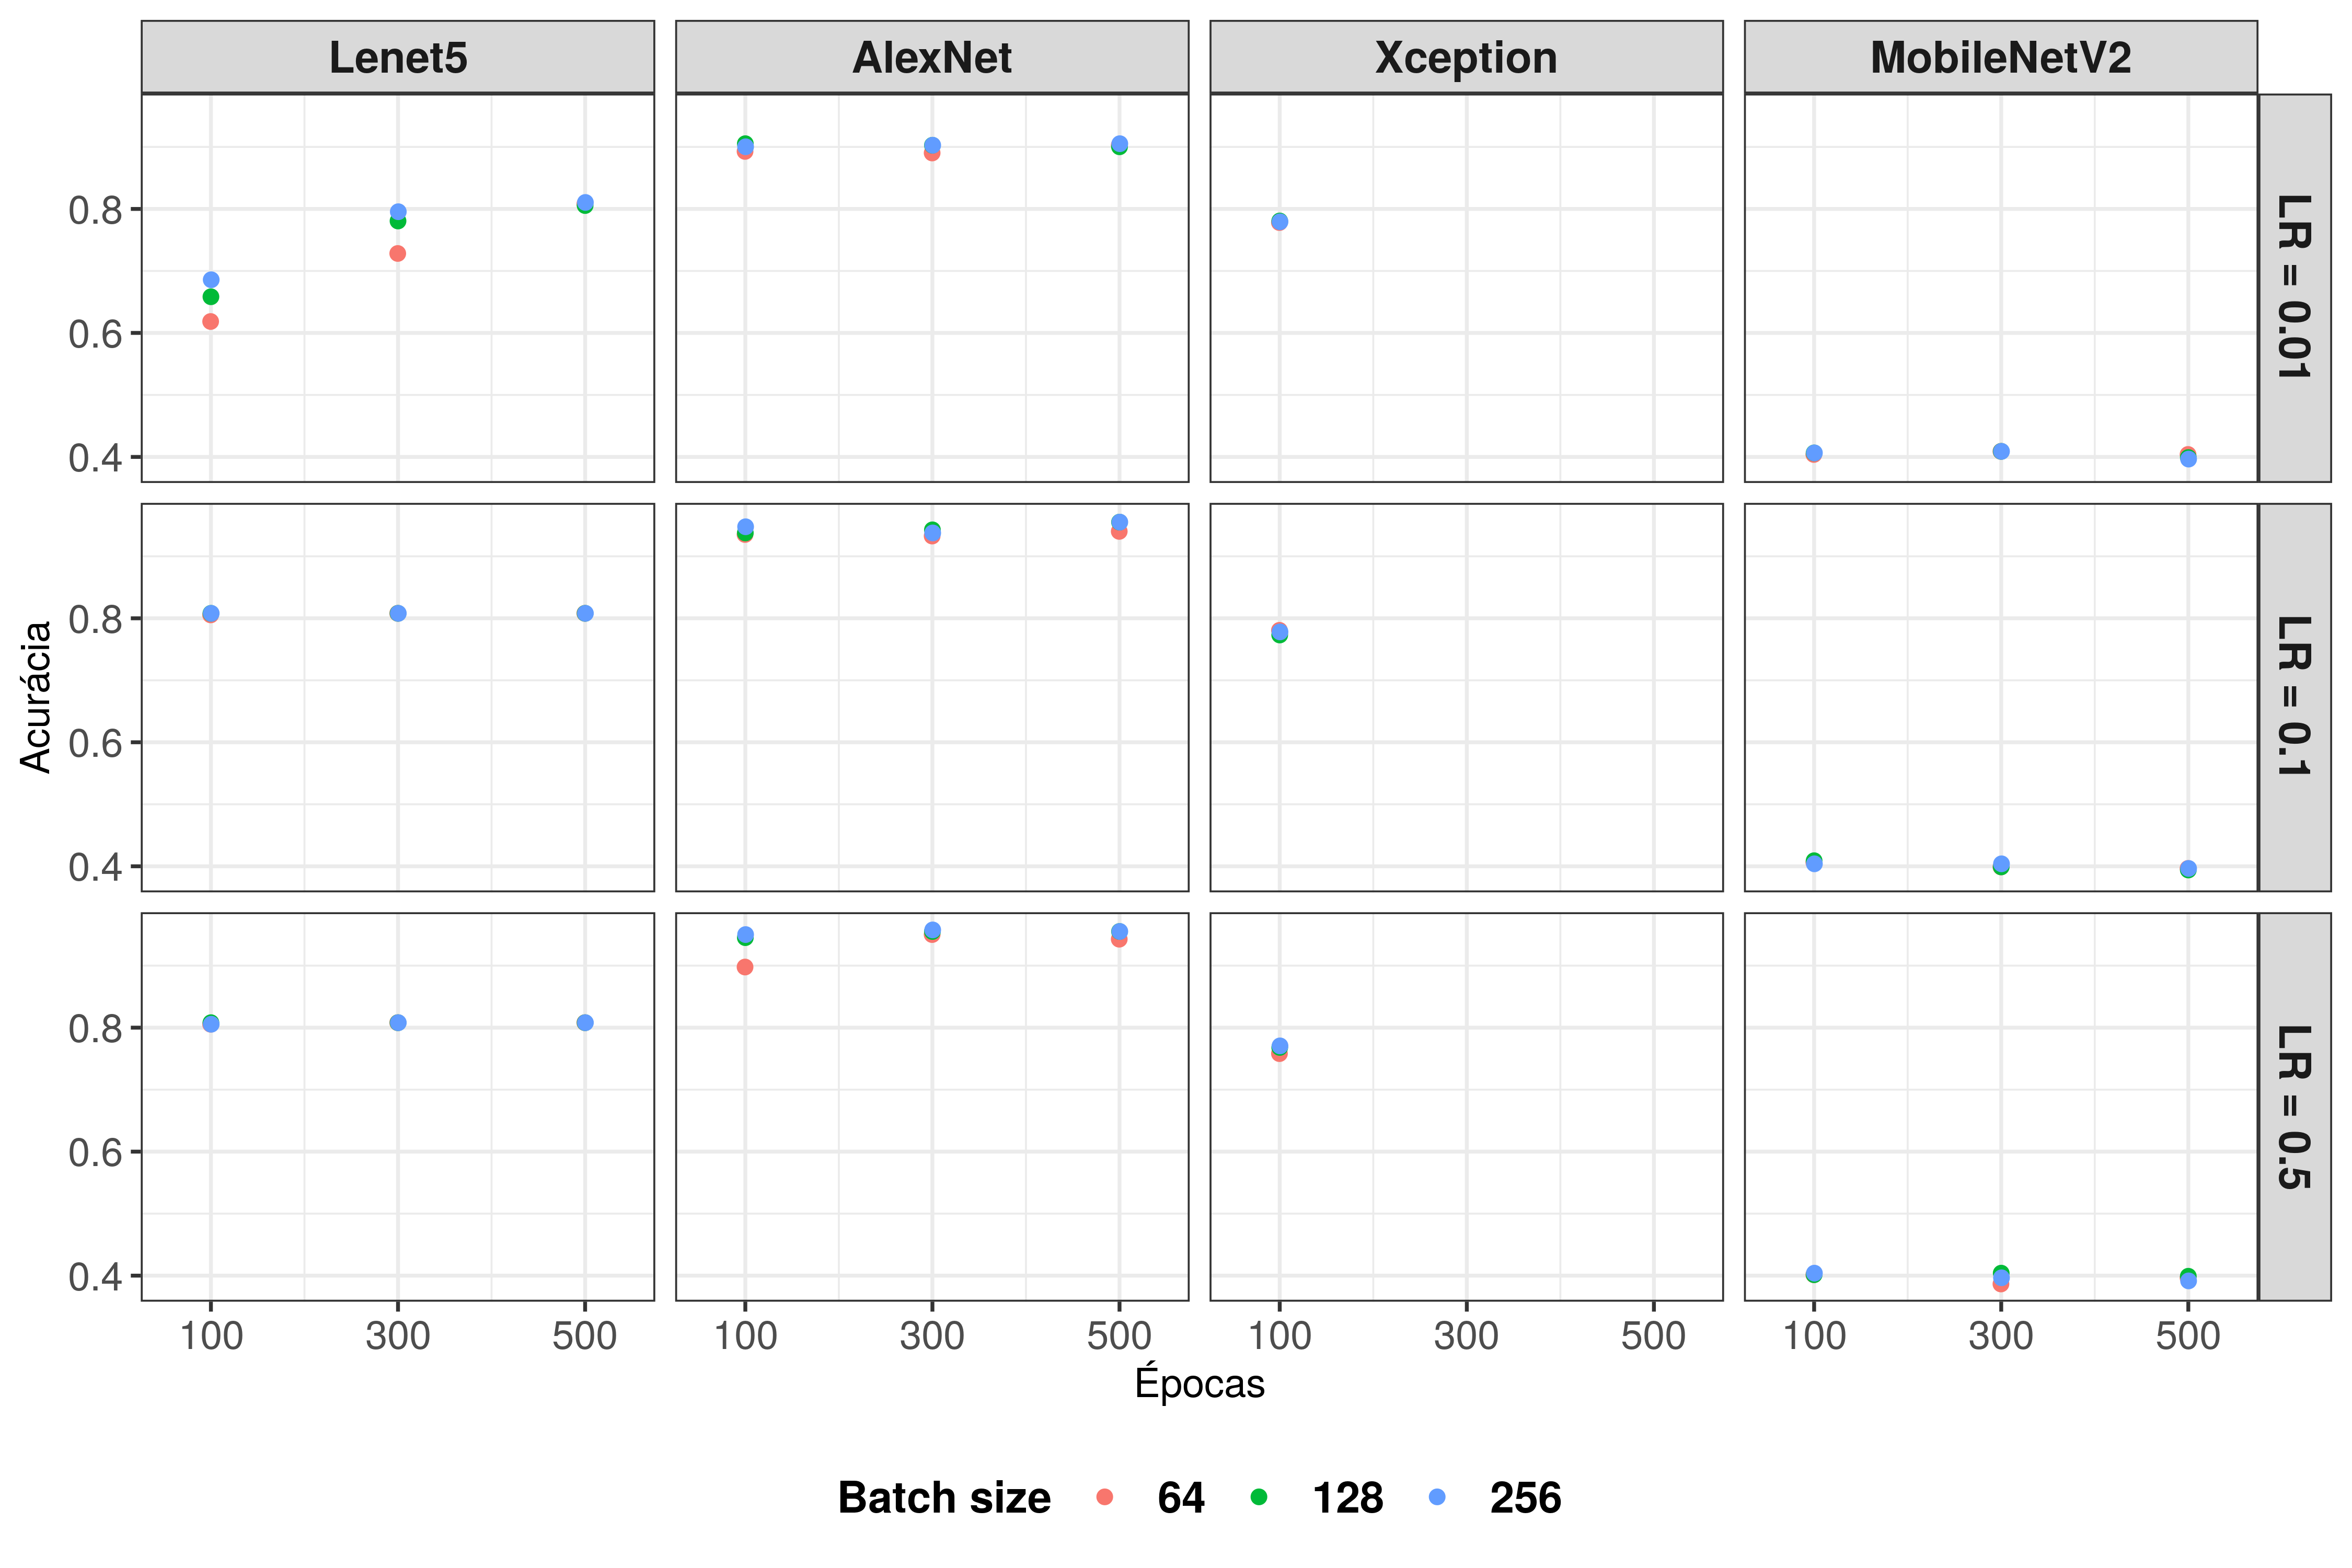
\includegraphics[width=1.6\textwidth]{/home/lacf14/machine_learning_ufpr/lab03/Analise/fig.png}
\caption{Acurácia observada para cada combinação do experimento.}
\end{figure}
\end{landscape}
